\section{Paketstruktur}
Dieser Abschnitt beschreibt die strukturelle Gliederung des Projektes in einem Paketdiagramm.

Wir betrachten die Pakete \textit{Robot} und \textit{Server} getrennt, da es eine physikalische Trennung zwischen den Geräten gibt, auf denen die jeweiligen Pakete vorhanden sein müssen.

Im \textit{Common} Paket sind alle Klassen enthalten, die sowohl vom \textit{Robot} als auch vom \textit{Server} Paket genutzt werden. So sind in dieser Iterationsstufe lediglich die Datentypen \textit{Position} und die davon erbende \textit{Destination} enthalten. Eine Möglichkeit zur Untescheidung von \textit{Destinations} ist wichtig, da zwischen vom \textit{Server} zugeteilten \textit{Destinations} und vom \textit{Robot} selbst zugeteilten \textit{Chargern} unterschieden werden muss. Jegliche Klassen und Interfaces die für die Kommunikation zuständig gewesen wären, wurden in dieser Iterationsstufe nach Aufgabenstellung nicht modelliert.

Das Paket \textit{Robot} enthält das Paket \textit{HardwareInterfaces}, welches die Möglichkeiten schafft, die Hardwareschnittstellen des \textit{Robots} direkt anzusprechen. Das Paket \textit{RobotControl} enthält Klassen zur Steuerung und Speicherung des Zustandes des \textit{Robots}, sowie die Handler, die den Hardwareschnittstellen übergeben werden.

Der Server besitzt in dieser Iterationsstufe noch keine Hardwareschnittstellen und enthält daher lediglich Klassen zur Verwaltung der \textit{Robots} und den jeweiligen \textit{Destinations}.


\begin{figure}[H]
\centering
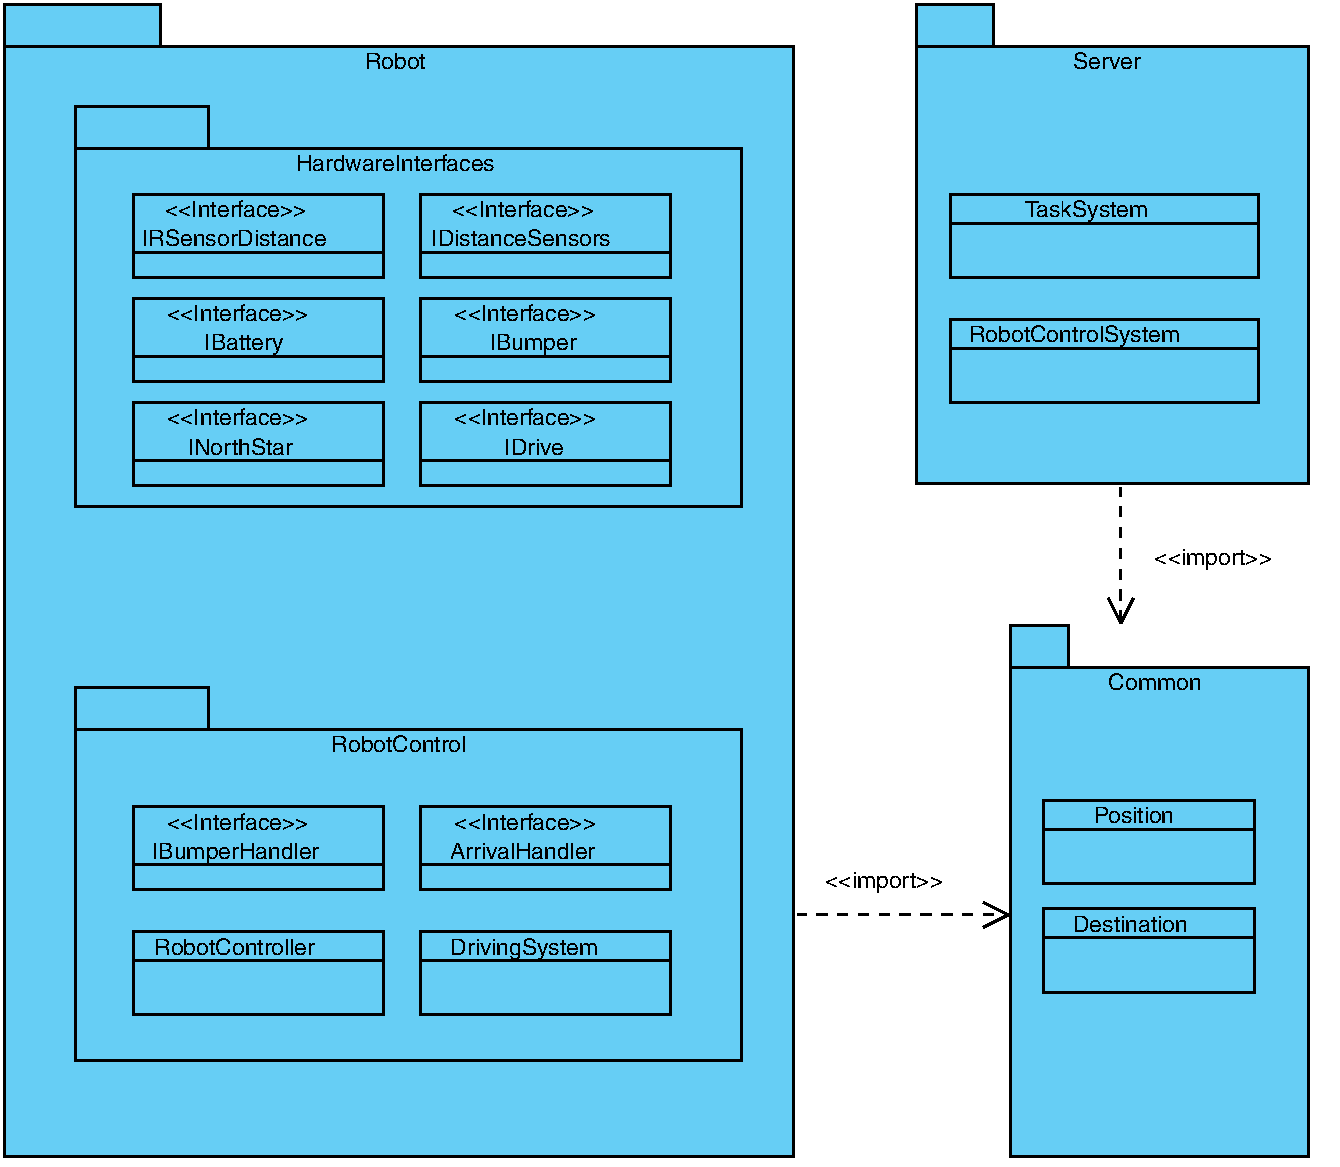
\includegraphics[width=0.8\textwidth]{../images/Iteration0_Entwurf_6_Paketdiagramm}
\caption{Paketdiagramm zur strukturellen Gliederung der Software}
\label{Paketstruktur}
\end{figure}